\section{eo\-Linear\-Truncate\-Split$<$ EOT $>$ Class Template Reference}
\label{classeo_linear_truncate_split}\index{eoLinearTruncateSplit@{eoLinearTruncateSplit}}
a Reduce\-Split class that does not sort, but repeatidely kills the worse.  


{\tt \#include $<$eo\-Reduce\-Split.h$>$}

Inheritance diagram for eo\-Linear\-Truncate\-Split$<$ EOT $>$::\begin{figure}[H]
\begin{center}
\leavevmode
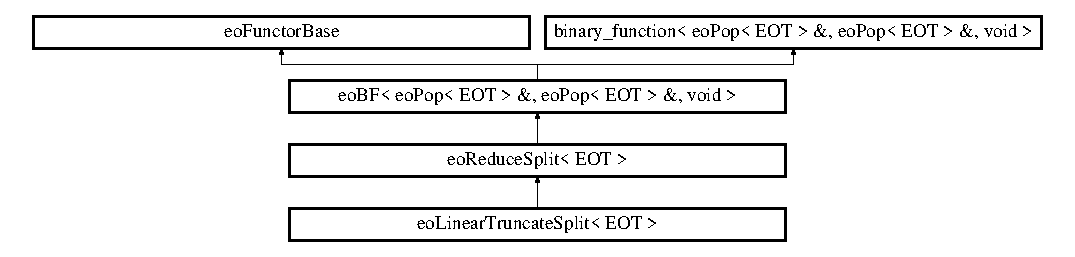
\includegraphics[height=3.01075cm]{classeo_linear_truncate_split}
\end{center}
\end{figure}
\subsection*{Public Member Functions}
\begin{CompactItemize}
\item 
{\bf eo\-Linear\-Truncate\-Split} ({\bf eo\-How\-Many} \_\-how\-Many, bool \_\-return\-Eliminated=false)\label{classeo_linear_truncate_split_a0}

\begin{CompactList}\small\item\em Ctor: must provide amount of reduction, and whether or not you need to return the eliminated guys. \item\end{CompactList}\item 
void {\bf operator()} ({\bf eo\-Pop}$<$ {\bf EOT} $>$ \&\_\-newgen, {\bf eo\-Pop}$<$ {\bf EOT} $>$ \&\_\-eliminated)\label{classeo_linear_truncate_split_a1}

\begin{CompactList}\small\item\em do the job \item\end{CompactList}\end{CompactItemize}
\subsection*{Private Attributes}
\begin{CompactItemize}
\item 
{\bf eo\-How\-Many} {\bf how\-Many}\label{classeo_linear_truncate_split_r0}

\item 
bool {\bf return\-Eliminated}\label{classeo_linear_truncate_split_r1}

\end{CompactItemize}


\subsection{Detailed Description}
\subsubsection*{template$<$class EOT$>$ class eo\-Linear\-Truncate\-Split$<$ EOT $>$}

a Reduce\-Split class that does not sort, but repeatidely kills the worse. 

To be used in SSGA-like replacements (e.g. see {\bf eo\-SSGAWorse\-Replacement}{\rm (p.\,\pageref{classeo_s_s_g_a_worse_replacement})}) 



Definition at line 87 of file eo\-Reduce\-Split.h.

The documentation for this class was generated from the following file:\begin{CompactItemize}
\item 
eo\-Reduce\-Split.h\end{CompactItemize}
